






% =========----------	[ Space left here for distraction free mode] ----------==========%









\subsection{Analysis 4: Is there a difference in perception of timbre with difference viewing positions?}
\label{ana4}
		
	The effect of different viewing positions on participants perception of timbre can be assessed by comparing the data collected for microphones that were shared across both viewing positions which includes the spot microphones and microphone arrays from position C. Figure~\ref{image:ta_sharedmics} shows the percentage of participants that selected each timbral attribute for each microphone. Table~\ref{ana4:barData} presents the corresponding data showing the percentage difference between each microphone pair (each microphone at both positions) calculated by subtracting the results for microphones at position B from the same microphones at position A. For each timbral attribute, the average results column indicates whether the attribute was selected by more participants for viewing position A (positive number) or position B (negative number). By looking at the table it can be seen that across all microphones the timbral attributes 'Realistic' and 'Loud' share the trend that they were selected by an equal or greater percentage of participants for viewing position A. The timbral attribute 'Realistic' experienced the greatest variation between viewing positions with an average difference of 19\%. Though the increased frequency of participants selecting 'Loud' is only by a minor amount, it is possible that the consistency is caused simply by the fact that viewing position A is closer to the musicians thus increasing the possibility for participants to perceive the audio as 'Loud'. \\

	\begin{figure}
		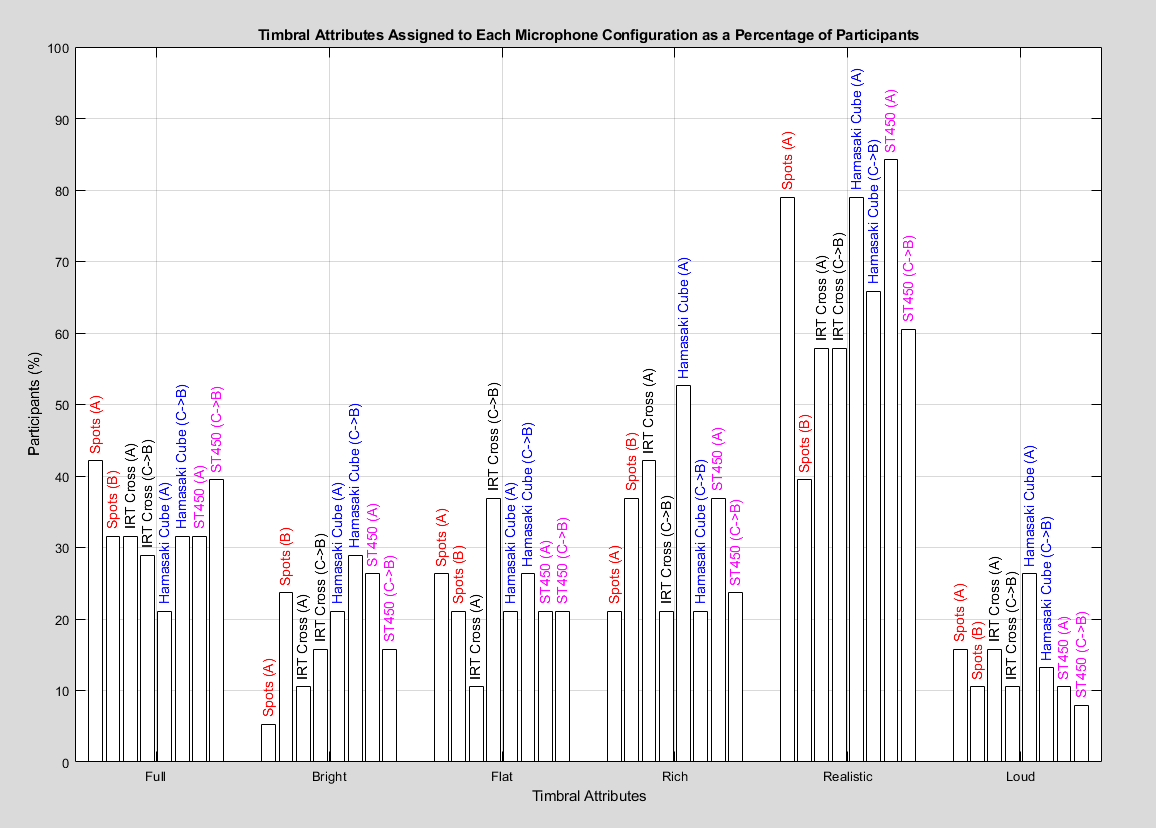
\includegraphics[width=\linewidth]{images/plots/bar_sharedMics.PNG}
		\caption{Bar chart showing the timbral attributes chosen for each microphone array shared between viewing position A and B as a percentage of participants}
		\label{image:ta_sharedmics} 
	\end{figure}	

	\begin{table}[h]
	\centering
	\resizebox{\linewidth}{!}{%
	\hspace{-15pt}
		\begin{tabular}{|>{\cen}m{15mm} |>{\cen}m{9.1mm} |>{\cen}m{9.5mm}| >{\cen}m{15mm}| *{2}{>{\cen}m{8mm}|}} \hline
		\multicolumn{1}{|>{\cen}m{12mm}|}{\multirow{2}{*}{Attributes}} & \multicolumn{4}{c|}{Microphones (\%)} & \multicolumn{1}{c|}{\multirow{2}{*}{\textbf{Averaged}}} \\ \cline{2-5}
		& Spots & IRT Cross & Hamasaki Cube & ST450 & \\ \hline
		Full & 10.53 & 2.63 & -10.53 & -7.89 & -1.32  \\ \hline
		Bright & -18.42 & -5.26 & -7.89 & 10.53 & -5.26 \\ \hline
		Flat & 5.26 & -26.32 & -5.26 & 0 & -6.58 \\\hline
		Rich & -15.79 & 21.05 & 31.59 & 13.16 & 12.5 \\ \hline
		Realistic & 39.47 & 0 & 13.16 & 23.68 & 19.08 \\ \hline
 		Loud & 5.2 & 5.2 & 13.16 & 2.63 & 6.58 \\ \hline
		\end{tabular}}
		\caption{Table showing the percentage difference between each pair of microphones calculated by $A - B$}
		\label{ana4:barData}
	\end{table}



	\textbf{Conclusion} \\

		In terms of timbre there appears to be little difference made by watching the performance from either position. The attributes effected most by changing viewing positions are a sense of whether things sounded realistic for which position A showed a preference. This increased difference however is mostly influenced by the large difference in spot microphone scores where there is a 39.5\% increase from the low 39.5\% of participants regarding the spot mics at position B to sound realistic to the 79\% of participants regarding the spot mics at position A to sound realistic. 

		It is hypothesised by the author that this is due to the unnatural lack of room acoustics heard when positioned at a distance where the sound of the room is expected to be heard. As the participant is standing much closer to the musicians at position A where the direct to reverb ratio is naturally much higher, the lack of room acoustics may be less noticeable and still be perceived as realistic. As a consequence of a lack of room acoustics present in the spot microphone mix, sound sources can be perceived more spatially isolated from one another. The unnaturalness of this is possibly less obvious when fully surrounded by the musicians as experienced at position A as this introduces an unnatural separation of the musicians for a listening experience. When viewing from position B however, as the musicians can be seen closer together, the unnatural sound source separation perceived may stand out to participants and further affect their judgement. \\


	% \begin{center}
	% \begin{table}
	% 	\begin{tabular}{r >{\centering\arraybackslash}p{30mm} c}
	% 		Attribute & Absolute Average Percentage Difference & Sway \\
	% 		Full & 7.89 & -1.32 \\
	% 		Bright & 10.53 & -5.26 \\
	% 		Flat & 9.21 & -6.58 \\
	% 		Rich & 20.39 & 12.5 \\
	% 		Realistic & 19.08 & 19.08 \\
	% 		Loud & 6.58 & 6.58 
	% 	\end{tabular}
	% 	\caption{Percentage difference}
	% 	\label{ana4:perDiff}
	% \end{table}
	% \end{center}